\documentclass[12pt, a4paper]{article}
\usepackage[top=3cm, bottom=3cm, left=3cm, right=3cm]{geometry}
\usepackage[T1]{fontenc}
\usepackage[utf8]{inputenc}
\usepackage[bahasa]{babel}
\usepackage{times}
\usepackage{graphicx}
\usepackage{amsmath, amssymb}
\usepackage{booktabs}
\usepackage{longtable}
\usepackage{enumitem}
\usepackage{hyperref}
\usepackage[round,authoryear]{natbib}
\usepackage{float}
\usepackage{setspace}

\hyphenation{Trans-for-mer En-co-der De-co-der me-nya-ma-kan in-fra-struk-tur cross-at-ten-tion meng-a-ko-mo-da-si}
\onehalfspacing

\setlength{\parindent}{1.25cm}
\setlength{\parskip}{0pt}

\begin{document}

\begin{center}
    \textbf{\Large CNN–Transformer Encoder–Decoder untuk Analisis Kuantitatif LIBS: Dekomposisi Spektral Mono–Poliatomik Eksplisit pada Karakterisasi Tanah Vulkanik}
\end{center}
\vspace{0.5cm}

\section*{Ringkasan}
\addcontentsline{toc}{section}{Ringkasan}
Laser-Induced Breakdown Spectroscopy (LIBS) merupakan teknik spektroskopi emisi yang memungkinkan analisis multi-elemen secara cepat tanpa memerlukan preparasi sampel yang kompleks. Meskipun pendekatan \textit{Calibration-Free LIBS} (CF-LIBS) memungkinkan kuantifikasi unsur tanpa standar rujukan eksternal, akurasinya sangat sensitif terhadap penyimpangan asumsi \textit{Local Thermodynamic Equilibrium} (LTE), terutama efek matriks berupa penyerapan mandiri (\textit{self-absorption}) dan gradien spasial plasma saat diaplikasikan pada material heterogen seperti tanah vulkanik. Di sisi lain, pendekatan \textit{machine learning} yang ada memperlakukan spektrum LIBS sebagai \textit{single composite signal}, mengabaikan fakta fisik fundamental bahwa spektrum poliatomik sejatinya merupakan superposisi terbobot konsentrasi dari spektrum monoatomik penyusunnya. Belum ada riset yang secara eksplisit memodelkan dekomposisi mono$\rightarrow$poliatomik dalam kerangka pembelajaran.

Penelitian ini mengusulkan arsitektur CNN–Transformer Encoder–Decoder yang secara struktural memodelkan hubungan dekomposisi spektral. Encoder memproses spektrum monoatomik individual yang dibangkitkan oleh Saha–Boltzmann \textit{forward model} untuk mempelajari representasi laten per-elemen melalui \textit{self-attention}. Decoder menerima spektrum campuran poliatomik dan memprediksi konsentrasi elemen melalui mekanisme \textit{cross-attention} terhadap output encoder, sehingga mempelajari aturan komposisi spektral secara \textit{end-to-end}. Lapisan 1D-CNN mengekstraksi fitur profil emisi lokal sebelum Transformer menangkap dependensi panjang gelombang global.

Model akan di-\textit{pre-train} pada spektrum sintetis yang dibangkitkan dari transisi NIST Atomic Spectra Database dan di-\textit{fine-tune} pada pengukuran LIBS eksperimental pada sampel tanah vulkanik dari Aceh, Indonesia, dengan data X-ray Fluorescence (XRF) sebagai \textit{ground-truth} konsentrasi. Perbandingan \textit{baseline} dilakukan terhadap model CNN-only, Transformer-only, Partial Least Squares, dan Informer. Kontribusi penelitian ini meliputi: (i) framework encoder–decoder yang memisahkan representasi spektral mono/poliatomik secara struktural, (ii) mekanisme \textit{cross-attention} untuk regresi konsentrasi yang \textit{physically interpretable}, dan (iii) aplikasi pada matriks tanah vulkanik kompleks Aceh, Indonesia.

\vspace{0.3cm}
\noindent \textbf{Kata Kunci}: LIBS; \textit{deep learning}; CNN–Transformer; encoder–decoder; \textit{cross-attention}; dekomposisi spektral; tanah vulkanik

\newpage
\tableofcontents
\newpage

\section{Pendahuluan}

\subsection{Latar Belakang}
Laser-Induced Breakdown Spectroscopy (LIBS) merupakan teknik spektroskopi emisi yang telah banyak digunakan untuk analisis komposisi unsur pada berbagai material kompleks, termasuk mineral, batuan, dan material tanah \citep{legnaioli2025}. Kemampuan LIBS untuk melakukan analisis multi-elemen secara cepat tanpa memerlukan preparasi sampel yang kompleks menjadikannya metode yang menarik untuk aplikasi geokimia dan eksplorasi sumber daya alam \citep{sawyers2025}. Berbagai penelitian menunjukkan bahwa LIBS telah berhasil digunakan untuk kuantifikasi unsur pada sampel geologi melalui beragam pendekatan analitik, mulai dari regresi multivariat, kurva kalibrasi univariat berbasis garis spektral tertentu \citep{zhang2025}, hingga metode berbasis \textit{machine learning} \citep{babos2024, manzoor2025}. Pendekatan-pendekatan tersebut mampu mencapai akurasi analitik yang tinggi, namun keberhasilan kuantifikasi sangat bergantung pada strategi pemodelan spektrum serta sensitivitas metode terhadap efek matriks pada sampel geologi yang kompleks \citep{hao2024, manelski2024}. Kondisi ini menjadi semakin relevan pada analisis tanah vulkanik, yang secara inheren memiliki komposisi multi-elemen dengan variasi matriks yang tinggi.

Dalam pendekatan kuantitatif LIBS, salah satu metode yang banyak digunakan adalah \textit{Calibration-Free LIBS} (CF-LIBS), yang memungkinkan estimasi komposisi unsur tanpa memerlukan sampel standar kalibrasi. Metode ini bergantung pada ekstraksi parameter plasma fundamental seperti temperatur elektron ($T_e$) dan densitas elektron ($n_e$), yang dihitung berdasarkan asumsi \textit{Local Thermodynamic Equilibrium} (LTE) \citep{cristoforetti2010}. Namun, asumsi plasma homogen dalam kondisi LTE sering kali tidak memadai untuk mendeskripsikan plasma LIBS yang bersifat sangat transien dan bergradien tinggi \citep{zaitsev2024, bultel2025}. Penyimpangan dari kondisi LTE ini dapat memicu distorsi spektral akibat efek opasitas optik dan penyerapan mandiri (\textit{self-absorption}), yang pada akhirnya mengganggu stabilitas estimasi temperatur dan densitas plasma \citep{tang2024, hansen2021}. Pendekatan berbasis model fisika plasma seperti model \textit{radiative transfer} adaptif MERLIN \citep{favre2025a} yang memanfaatkan distribusi Saha–Boltzmann serta Persamaan Transfer Radiatif menunjukkan bahwa rekonstruksi spektrum LIBS yang kompleks dapat dicapai dengan mempertahankan konsistensi termodinamika plasma, meskipun implementasinya masih menghadapi hambatan komputasi yang signifikan akibat kebutuhan inversi numerik nonlinier \citep{favre2025b}.

Perkembangan metode \textit{machine learning} dan \textit{deep learning} telah menawarkan alternatif untuk mempercepat analisis spektrum LIBS dengan mempelajari hubungan nonlinier antara spektrum dan parameter plasma secara langsung dari data. \textit{Convolutional Neural Networks} (CNN) mampu menangkap fitur lokal seperti profil garis emisi, sementara arsitektur Transformer memodelkan dependensi jarak jauh sepanjang sumbu panjang gelombang \citep{liu2026}. Model hibrida CNN–Transformer telah menunjukkan hasil menjanjikan untuk kuantifikasi unsur jejak pada baja \citep{liu2026} dan untuk klasifikasi signatur spektral pada sampel multi-elemen \citep{walidain2026}. Namun, sebagian besar model \textit{data-driven} beroperasi sebagai \textit{black box} yang tidak secara eksplisit mempertimbangkan hukum fisika plasma yang mendasari pembentukan spektrum emisi \citep{hao2024}. Fakta fisik fundamental yang belum dieksploitasi adalah: spektrum LIBS poliatomik merupakan superposisi terbobot konsentrasi dari spektrum monoatomik penyusunnya. Seluruh model eksisting—baik berbasis fisika maupun \textit{data-driven}—memperlakukan spektrum sebagai \textit{single signal} dan mengabaikan struktur komposisional ini. \textbf{Belum ada penelitian sebelumnya yang secara eksplisit memodelkan dekomposisi spektrum campuran ke dalam konstituennya dalam kerangka pembelajaran.} \textit{Cross-attention}, mekanisme yang awalnya diusulkan untuk translasi sekuens-ke-sekuens \citep{vaswani2017}, sangat ideal untuk tugas ini: decoder dapat meng-\textit{query} representasi elemen dari encoder untuk mengetahui kontribusi monoatomik mana yang membentuk observasi poliatomik tertentu \citep{liu2026, walidain2026}.

\textbf{Penelitian ini mengusulkan arsitektur CNN–Transformer encoder–decoder yang memperkenalkan dekomposisi spektral mono–poliatomik eksplisit ke dalam analisis kuantitatif LIBS.} Encoder memproses spektrum monoatomik individual yang dibangkitkan oleh Saha–Boltzmann \textit{forward model} untuk mempelajari representasi laten spesifik-elemen. Decoder menerima spektrum campuran poliatomik dan memprediksi konsentrasi elemen melalui \textit{cross-attention} terhadap output encoder. Lapisan 1D-CNN mengekstraksi fitur emisi lokal sebelum Transformer menangkap dependensi panjang gelombang global. Model di-\textit{pre-train} pada spektrum sintetis dari NIST Atomic Spectra Database dan di-\textit{fine-tune} pada pengukuran LIBS eksperimental tanah vulkanik dari Aceh, Indonesia, dengan analisis XRF menyediakan \textit{ground-truth} konsentrasi.

\subsection{Rumusan Permasalahan yang Akan Diteliti}
\begin{enumerate}[label=\arabic*.]
    \item Bagaimana memodelkan hubungan antara spektrum poliatomik yang dihasilkan dari plasma LIBS dengan spektrum monoatomik penyusun yang merepresentasikan karakteristik unsur individual?
    \item Bagaimana merancang arsitektur pembelajaran mendalam yang mampu mengekstraksi fitur spektral lokal serta menangkap dependensi global antar panjang gelombang pada spektrum LIBS?
    \item Bagaimana memanfaatkan arsitektur CNN–Transformer encoder–decoder untuk mempelajari hubungan struktural antara spektrum monoatomik dan spektrum poliatomik dalam analisis spektrum LIBS?
    \item Bagaimana kinerja model yang diusulkan dalam memprediksi konsentrasi unsur serta parameter plasma dari spektrum LIBS pada sampel tanah vulkanik?
\end{enumerate}

\subsection{Pendekatan Pemecahan Masalah}
Untuk mengatasi tantangan inferensi parameter komposisi akibat kompleksitas \textit{matrix effect} dan opasitas pada tanah vulkanik, penelitian ini mengusulkan sebuah pendekatan pemodelan inversi memanfaatkan \textit{deep learning} yang \textit{physics-informed}. Pendekatan ini secara struktural memecahkan masalah tumpang-tindih (\textit{overlap}) spektrum dengan memodelkan dekomposisi superposisi spektral melalui arsitektur CNN-Transformer \textit{encoder-decoder}. Pendekatan ini beroperasi secara proaktif: \textit{encoder} merepresentasikan basis spektral monoatomik yang dibangkitkan via \textit{forward model} Saha-Boltzmann, sedangkan \textit{decoder} menggunakan komputasi \textit{cross-attention} untuk memproyeksikan fraksi multielemen dari spektrum campuran poliatomik eksperimental secara simultan tanpa bergantung pada kurva kalibrasi konvensional.

\subsection{Tujuan Khusus Penelitian}
\begin{enumerate}[label=\arabic*.]
    \item Memodelkan komposisi spektral melalui arsitektur encoder–decoder yang secara eksplisit memodelkan hubungan antara spektrum monoatomik (representasi per-elemen) dan spektrum poliatomik (campuran terukur).
    \item Mengembangkan arsitektur hibrida CNN–Transformer yang menggabungkan ekstraksi fitur lokal (CNN 1D untuk profil puncak emisi) dan pemodelan dependensi global (Transformer untuk korelasi antar panjang gelombang) dalam paradigma encoder–decoder.
    \item Memprediksi konsentrasi unsur secara akurat pada sampel tanah vulkanik dari Aceh dan mengevaluasi kinerja model terhadap baseline (PLS, CNN-only, Transformer-only, Informer).
\end{enumerate}

% Bagian kebaruan ini dipindahkan ke State-of-the-Art dan Kebaruan

\subsection{State-of-the-Art dan Kebaruan}

\subsubsection{Kajian \textit{State-of-the-Art}}
Penelitian analisis geokimia material geologi dari wilayah Aceh dan Indonesia telah menjadi fokus utama terstruktur dari grup riset ini secara berkelanjutan. Dimulai dari evaluasi prekursor sejak tahun 2021, grup riset telah membuktikan kapabilitas *TEA CO2* LIBS dalam mengkarakterisasi komponen kimia tanah terdampak tsunami raksasa Samudra Hindia 2004 secara berkesinambungan \citep{sari_new_2021}. Upaya pemetaan komprehensif ini diperkuat dengan pendekatan multi-instrumen yang melibatkan validasi silang menggunakan *Scanning Electron Microscopy-Energy Dispersive X-ray* (SEM-EDX) \citep{sari_new_2021, ramli_elemental_2023-1} serta instrumen optik *X-Ray Fluorescence* (XRF) \citep{mitaphonna_x-ray_2023} guna memancang *ground-truth* proksi laut pada lapisan endapan di Provinsi Aceh.

Memasuki fase eksplorasi selanjutnya, pencarian struktur kandidat endapan purba juga berhasil mengidentifikasi dan melokalisasi sedimen preservasi tsunami secara fisik di kawasan strategis terdampak di Aceh Besar, khususnya Desa Pulot \citep{mitaphonna_characteristics_2023} dan Desa Seungko Meulat \citep{mitaphonna_preliminary_2024}. Ekstraksi *chemical profile* memanfaatkan rekayasa plasma bertekanan atmosferik (*TEA CO2 laser*) \citep{mitaphonna_characteristics_2023, mitaphonna_pulsed_2024} serta *Nd:YAG LIBS* standar \citep{mitaphonna_pulsed_2024} berhasil mengidentifikasi keberadaan elemen-elemen mayor laut seperti Si, Al, Fe, Ca, Mg, Na, dan K secara tegas pada matriks sampel geo-sedimen. Ekspansi peta jalan penelitian eksperimental ini menunjukkan bahwa instrumen LIBS sonder resolusi (*stand-alone*) sangat kapabel dalam mendeteksi signatur endapan poliatom. Namun, kapabilitas analisis mutakhir ini \textbf{masih membatasi diri pada ekskavasi kualitatif}—yang menjustifikasi urgensi krusial untuk melahirkan pendekatan analitik kuantitatif baru menggunakan kecerdasan buatan (*deep learning*).

Pada skala nasional, Khumaeni, Idris et al. (2025) \citep{khumaeni_analysis_2025} mendemonstrasikan penerapan CF-LIBS untuk analisis komposisi geokimia dan mineral tanah vulkanik yang terdampak erupsi Gunung Merapi di Jawa Tengah. Studi ini membuktikan bahwa CF-LIBS \textbf{dapat} diterapkan pada tanah vulkanik Indonesia, namun sekaligus mengekspos keterbatasan inherennya: akurasi bergantung pada validitas asumsi LTE yang sering dilanggar pada matriks tanah vulkanik yang sangat heterogen. Keterbatasan ini menjadi motivasi langsung untuk pengembangan pendekatan berbasis \textit{deep learning} yang diusulkan dalam tesis ini.

Dalam lanskap komputasi LIBS global, perkembangan penelitian telah berevolusi dari simulasi fisika murni menuju integrasi \textit{machine learning} dan \textit{deep learning}:

\textbf{Favre et al. (2025)} \citep{favre2025b} mengembangkan pendekatan ML CF-LIBS kuantitatif yang memanfaatkan ekstraksi fitur CNN dari database simulasi berskala besar. Pendekatan ini terbukti ampuh untuk diagnostik simultan tanpa rekalibrasi, namun performa baseline-nya \textbf{kolaps pada percampuran puncak \textit{dense overlap}} yang umum dijumpai pada spektrum tanah vulkanik. Hal ini menunjukkan kebutuhan akan mekanisme kompensasi yang lebih canggih.

\textbf{Wang et al. (2024)} \citep{wang2024} mengusulkan hibridisasi pra-filter \textit{wavelet} dengan arsitektur Transformer dan CNN untuk analisis spektral berbantuan simulasi. Pendekatan ini mantap memadukan ikatan \textit{global dependency} dan deteksi pendaran lokal, namun \textbf{celah overlap fisik garis emisi tetap diabaikan} dan diperlakukan sebagai \textit{single signal} statis.

\textbf{Liu et al. (2026)} \citep{liu2026} memperkenalkan hibridisasi CNN–Transformer untuk LIBS jarak jauh (\textit{remote} LIBS) pada analisis unsur baja. Arsitektur ini berhasil menggabungkan deteksi pola lokal (CNN) dan dependensi global (Transformer), namun spektrum tetap diperlakukan sebagai \textbf{single composite signal} tanpa mempertimbangkan struktur komposisi spektral mono–poliatomik.

\textbf{Walidain et al. (2026)} \citep{walidain2026} mengadaptasi arsitektur Informer (\textit{ProbSparse attention}) untuk klasifikasi spektral LIBS pada sampel geologi. Studi ini membuktikan bahwa mekanisme \textit{attention} yang efisien mampu memproses spektrum LIBS bersekuens ultra-panjang, namun \textbf{hanya mencapai klasifikasi kualitatif}, bukan regresi kuantitatif konsentrasi.

\subsubsection{Kesimpulan \textit{Research Gap}}
\textbf{Observasi kunci}: Semua pendekatan di atas memperlakukan spektrum sebagai \textit{single signal}. Struktur komposisi spektrum LIBS — yaitu bahwa spektrum poliatomik merupakan superposisi dari spektrum monoatomik penyusun — belum pernah dieksplorasi secara eksplisit. Tidak ada penelitian sebelumnya yang: (i) memisahkan spektrum monoatom vs poliatom, (ii) menggunakan mekanisme \textit{attention} lintas komposisi, maupun (iii) menerapkan kerangka encoder–decoder untuk LIBS. Oleh karena itu, penelitian ini mengusulkan pendekatan di mana encoder mempelajari representasi monoatom, decoder merekonstruksi komposisi poliatom via \textit{cross-attention}, dan prediksi konsentrasi unsur dilakukan secara end-to-end.

\subsubsection{Kebaruan (\textit{Novelty}) Penelitian}
Kompensasi atas gap riset tersebut memastikan bahwa \textbf{kebaruan} dalam tesis ini meliputi:
\begin{enumerate}[label=\arabic*.]
    \item \textbf{Pemodelan spektral mono–poliatomik}: Pendekatan pertama yang secara eksplisit memodelkan hubungan komposisi antara spektrum monoatom dan poliatom LIBS melalui mekanisme \textit{cross-attention}.
    \item \textbf{Kerangka CNN–Transformer untuk analisis LIBS}: Arsitektur hibrida yang menggabungkan ekstraksi fitur lokal (CNN) dan pemodelan dependensi global (Transformer) dalam paradigma encoder–decoder.
    \item \textbf{Karakterisasi tanah vulkanik}: Prediksi kuantitatif konsentrasi unsur pada matriks geologi kompleks, relevan untuk vulkanologi dan penilaian tanah pertanian.
\end{enumerate}

\subsection{Peta Jalan (\textit{Roadmap}) Penelitian}
\begin{figure}[htbp]
    \centering
    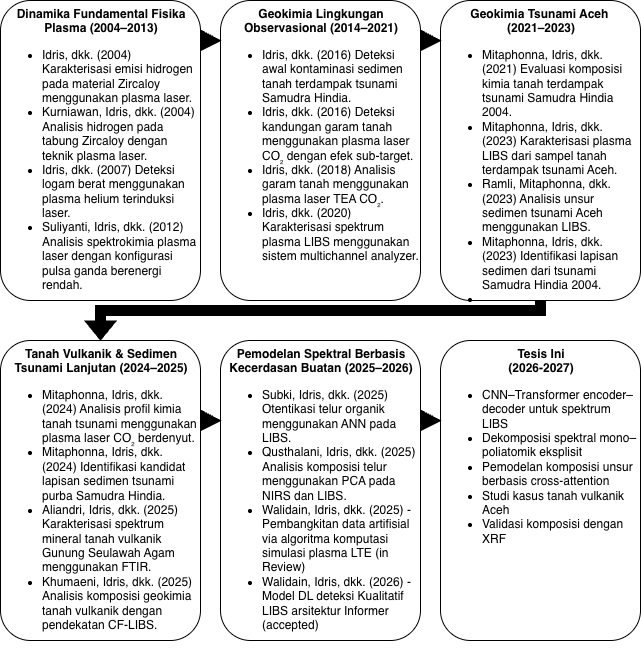
\includegraphics[width=1\textwidth]{Peta-Grup.png}
    \caption{Peta jalan penelitian menunjukkan progresi dari fondasi riset grup menuju riset AI spektral LIBS mutakhir.}
    \label{fig:roadmap}
\end{figure}

\begin{table}[htbp]
\centering
\caption{Ringkasan Historis Peta Jalan (\textit{Roadmap}) Evolusi Riset Grup Pemandu}
\label{tab:roadmap_historis}
\renewcommand{\arraystretch}{1.5}
\begin{tabular}{@{} l p{4.5cm} p{6cm} p{3.5cm} @{}}
\toprule
\textbf{Fase/Tahun} & \textbf{Fokus \& Tema Utama} & \textbf{Capaian Ilmiah Utama (\textit{Milestone})} & \textbf{Sitasi Basis} \\ \midrule

\textbf{Tahap I} & \textbf{Dinamika Fundamental Fisika Plasma} & 
Karakterisasi awal \textit{Laser-Induced Shock Wave Plasma}, eksitasi pada lingkungan tekanan rendah, dan analisis fisis deuterium/hidrogen pada padatan keras seperti pipa reaktor (\textit{Zircaloy-4}). & 
Idris et al. (2004), Idris et al. (2013) \\ \midrule

\textbf{Tahap II} & \textbf{Transisi Aplikasi: Sedimen \& Geokimia} & 
Penerapan LIBS untuk mengekstraksi dan mendeteksi kontaminasi jejak elemen pada sedimen tanah sisa Tsunami Aceh 2004 menggunakan instrumen laser TEA CO$_2$ dan Nd:YAG. & 
Idris et al. (2016), Idris et al. (2019) \\ \midrule

\textbf{Tahap III} & \textbf{Resolusi Validasi Lintas-Instrumen} & 
Analisis interdisiplin melalui silang-validasi proksi Paleo-tsunami dan geokimia tanah laut menggunakan instrumen baku tambahan seperti SEM-EDX dan mesin X-Ray Fluorescence (XRF). & 
Mitaphonna (2021), Idris et al. (2023) \\ \midrule

\textbf{Tahap IV} & \textbf{Modernisasi \textit{AI} \& Kuantifikasi Spektral} & 
\textit{(Fokus Tesis)} Mengatasi limitasi kualitatif dan \textit{matrix effect} tanah melalui pendekatan sintesis arsitektur \textit{Deep Learning} otomatis (Model regresi \textit{CNN-Transformer}). & 
Wang (2024), Walidain dkk. (2026) \\ \bottomrule
\end{tabular}
\vspace{2mm} % Space between table and source note
\par
\textit{Sumber: Tinjauan sistematis atas 100 literatur Nasrullah Idris \textit{et al.} dari Semantic Scholar (2004--2024), dirumuskan mandiri.}
\end{table}


Peta jalan (Gambar~\ref{fig:roadmap}) menggambarkan trajektori evolusi riset grup selama dua dekade, yang terbagi dalam lima fase berdasarkan pergeseran tema penelitian.

\textbf{Fase I -- Dinamika Fundamental Fisika Plasma (2004--2013).}
Fase ini merupakan fondasi spektroskopi plasma laser grup riset. Fokus utama diarahkan pada karakterisasi emisi hidrogen dan deuterium pada material eksotis seperti bahan bakar reaktor nuklir (\textit{Zircaloy-4}), menggunakan laser TEA CO\textsubscript{2} dan Nd:YAG dalam lingkungan gas helium tekanan rendah \citep{idris_characteristics_2004, kurniawan_hydrogen_2004}. Studi awal ini membuktikan kemampuan LIBS dalam mendeteksi elemen-elemen ringan dan logam berat \citep{idris_analysis_2007}, serta meletakkan dasar teknis konfigurasi pulsa ganda berenergi rendah yang menjadi ciri khas pendekatan instrumentasi grup \citep{colao_quarry_2010}.

\textbf{Fase II -- Geokimia Lingkungan Observasional (2014--2021).}
Kompetensi analitik plasma laser yang telah matang kemudian diarahkan ke objek geokimia lingkungan. Tonggak penting fase ini adalah deteksi awal kontaminasi sedimen tanah yang terdampak gelombang Tsunami Samudra Hindia 2004 di wilayah Aceh \citep{idris_excitation_2015}. Grup mengembangkan metode kuantifikasi garam tanah pesisir pertanian dengan memanfaatkan efek \textit{sub-target} unik pada plasma laser CO\textsubscript{2} \citep{sari_investigation_2020}, serta mengembangkan teknik analisis menggunakan sistem TEA CO\textsubscript{2} berenergi rendah \citep{idris_detection_2018}. Fase ini ditutup dengan karakterisasi komprehensif spektrum LIBS menggunakan sistem \textit{optical multichannel analyzer} portabel \citep{idris_geochemistry_2022-1}.

\textbf{Fase III -- Geokimia Tsunami Aceh (2021--2023).}
Fase ini menandai dedikasi penuh grup pada kajian saintifik mendalam atas tanah terdampak Tsunami Aceh 2004. Dimulai dari evaluasi komposisi kimia tanah menggunakan laser CO\textsubscript{2} \citep{sari_new_2021}, dilanjutkan dengan studi geokimia komprehensif menggunakan Nd:YAG harmonik-keempat \citep{idris_geochemistry_2022}. Grup kemudian melakukan karakterisasi plasma dari sampel sedimen tsunami menggunakan TEA CO\textsubscript{2} \citep{mitaphonna_characteristics_2023} dan analisis elemental kuantitatif sedimen tsunami Aceh via LIBS \citep{ramli_elemental_2023-1}. Puncak fase ini adalah identifikasi kandidat lapisan paleotsunami menggunakan \textit{X-Ray Fluorescence} (XRF) sebagai instrumen silang-validasi \citep{mitaphonna_x-ray_2023}.

\textbf{Fase IV -- Tanah Vulkanik \& Sedimen Tsunami Lanjutan (2024--2025).}
Fase ini mencerminkan perluasan kapabilitas analitik grup ke objek material geologis yang lebih beragam. Analisis profil kimia tanah tsunami secara mendalam menggunakan sistem plasma laser CO\textsubscript{2} berdenyut dilakukan oleh Mitaphonna dkk.\ \citep{mitaphonna_pulsed_2024}. Secara paralel, identifikasi kandidat lapisan sedimen purba Tsunami 2004 di wilayah Seungko Meulat terus diperluas \citep{mitaphonna_preliminary_2024}. Dua studi baru turut membuka dimensi vulkanologi: karakterisasi spektrum mineral FTIR dari tanah vulkanik Gunung Seulawah Agam \citep{aliandri_evaluation_2025}, serta analisis komposisi geokimia tanah letusan Gunung Merapi menggunakan pendekatan \textit{calibration-free} LIBS \citep{khumaeni_analysis_2025}.

\textbf{Fase V -- Pemodelan Spektral Berbasis Kecerdasan Buatan (2025--2026).}
Fase kelima menandai modernisasi metodologis grup melalui integrasi kecerdasan buatan dan komputasi fisika. Studi otentikasi telur organik menggunakan ANN (\textit{Artificial Neural Networks}) \citep{subki_analysis_2025} dan komparasi spektrum cangkang telur dengan NIRS via analisis komponen utama (PCA) \citep{qusthalani_comparing_2025} membuktikan skalabilitas platform LIBS pada objek biologis. Secara bersamaan, riset komputasi Walidain et al.\ memperkenalkan paradigma baru berupa pembangkitan data sintetik berbasis simulasi fisika plasma LTE \citep{walidain_spectroscopic_2025} dan prediksi multi-elemen kualitatif menggunakan arsitektur \textit{Informer} berbasis \textit{deep learning} \citep{walidain_informer-based_2026}. Capaian Fase V ini secara langsung menjadi landasan dan motivasi bagi Tesis ini.

\textbf{Tesis Ini (2026--2027).}
Tesis ini merupakan puncak dari trajektori yang telah dibangun selama dua dekade. Mengintegrasikan pemahaman fisika plasma dari Fase I--IV dengan kompetensi komputasi dari Fase V, penelitian ini mengusulkan kerangka \textit{CNN--Transformer Encoder--Decoder} yang pertama kali menerapkan dekomposisi eksplis\-it mono-poliatomik pada spektrum LIBS. Objek yang dipilih adalah tanah vulkanik Gunung Seulawah Agam, Aceh, dengan validasi komposisi silang terhadap instrumen XRF.


\newpage

% ================================================================
%  PROFIL MAHASISWA
% ================================================================
\section{Profil Mahasiswa}
% TODO: Silakan tambahkan profil mahasiswa sesuai dengan format universitas (dilewatkan untuk saat ini).

\newpage

% ================================================================
%  METODE PENELITIAN
% ================================================================
\section{METODE PENELITIAN}

\subsection{Lokasi Penelitian}

Penelitian ini dilaksanakan dalam dua tahap utama yang mencakup kegiatan eksperimental dan komputasional. Tahap eksperimental meliputi preparasi sampel yang dilakukan di \textbf{Laboratorium Material, FMIPA Universitas Syiah Kuala}, serta akuisisi data spektrum LIBS yang dilaksanakan di \textbf{Laboratorium Optika dan Aplikasi Laser, FMIPA Universitas Syiah Kuala}. Laboratorium ini dilengkapi dengan sistem LIBS berbasis laser Nd:YAG dan spektrometer Echelle yang telah digunakan dalam berbagai studi spektroskopi sebelumnya \citep{mitaphonna_characteristics_2023, mitaphonna_pulsed_2024, khumaeni_analysis_2025}. Pengukuran komposisi unsur sebagai data referensi (\textit{ground-truth}) menggunakan instrumen X-Ray Fluorescence (XRF) dilakukan di fasilitas analisis yang tersedia di lingkungan Universitas Syiah Kuala.

Tahap komputasional---yang mencakup pembangkitan data sintetis, pengembangan arsitektur model CNN--Transformer encoder--decoder, serta seluruh siklus pelatihan dan evaluasi---dilaksanakan menggunakan \textbf{GPU Compute Server} yang tersedia di laboratorium penelitian. Keseluruhan penelitian direncanakan berlangsung selama \textbf{10 bulan}, dari Februari 2025 hingga November 2025, dengan rincian per fase disajikan pada bagian Jadwal Penelitian.


\subsection{Alat dan Bahan Penelitian}

Penelitian ini memadukan pendekatan fisika eksperimental optik dan komputasi \textit{machine learning}. Oleh karena itu, instrumen yang digunakan dikategorikan menjadi instrumen perangkat keras eksperimental, infrastruktur komputasi, perangkat lunak penunjang, serta sumber data.

\subsubsection{Instrumen Eksperimental dan Preparasi Sampel}
Peralatan eksperimen utama yang digunakan untuk pengadaan sampel tanah vulkanik dan penembakan spektral LIBS disajikan pada Tabel~\ref{tab:alat-bahan}.

\begin{table}[htbp]
\centering
\caption{Instrumen Eksperimental Material dan Optik}
\label{tab:alat-bahan}
\small
\begin{tabular}{clp{5.5cm}l}
\toprule
\textbf{No} & \textbf{Alat/Bahan} & \textbf{Spesifikasi} & \textbf{Jumlah} \\
\midrule
1  & Laser Nd:YAG              & Q-switched, $\lambda$ = 1064 nm, 114 mJ   & 1 unit \\
2  & Lensa bikonveks           & $f$ = 155 mm (pemfokusan laser)            & 1 unit \\
3  & Spektrometer Echelle + OMA& Rentang spektral 200--900 nm               & 1 unit \\
4  & Mesin \textit{hydraulic press} & Tekanan hingga 7 ton                  & 1 unit \\
5  & Mortar, Pestel, dan Ayakan& Penggerusan dan ayakan 40 mesh (420 $\mu$m) & 1 set  \\
6  & Instrumen XRF             & \textit{Ground-truth} kuantifikasi elemen  & 1 unit \\
7  & Sampel tanah vulkanik     & G. Seulawah Agam (4 arah $\times$ 3 kedalaman) & 24 sampel \\
\bottomrule
\end{tabular}
\end{table}

\subsubsection{Perangkat Keras Komputasi}
Untuk mengakomodasi kalkulasi dari pembuatan arsitektur \textit{deep learning} (CNN--Transformer) dan \textit{forward modeling} data sintetis, penelitian ini memerlukan kapabilitas komputasi berkinerja tinggi yang disokong oleh:
\begin{enumerate}
    \item \textbf{Laptop Apple MacBook Air M1 2020}: Dilengkapi dengan prosesor \textit{Apple M1}, memori (RAM) sebesar 8 GB, dan penyimpanan \textit{SSD}. Perangkat ini secara utama digunakan untuk pengembangan skrip kode lokal, eksplorasi matematis awal, dan penyusunan laporan akademis.
    \item \textbf{Infrastruktur \textit{High Performance Computing} (HPC) Mahameru 4 BRIN}: Infrastruktur ini digunakan secara masif untuk simulasi spektroskopi emisi sintetis berskala besar dan pelatihan model CNN--Transformer yang intensif secara komputasi. Spesifikasi komputasinya meliputi:
    \begin{itemize}
        \item \textbf{Klaster CPU}: 92 \textit{compute node} dengan dual prosesor Xeon Gold (sekitar 32 core per \textit{node}) dan 256 GB RAM per \textit{node}. Terdapat 1 \textit{high memory node} dengan kapasitas memori hingga 1.5 TB.
        \item \textbf{Klaster GPU}: Terkonsolidasi dari berbagai akselerator \textit{Graphics Processing Unit} kelas berat (di antaranya varian NVIDIA DGX A100, V100, dan P100).
        \item \textbf{Sistem Penyimpanan}: Kapasitas masif total 4.5 PB, didukung arsitektur \textit{High Performance SSD} untuk menampung matriks HDF5 berjuta-baris dengan efisien.
        \item \textbf{Jaringan Interkoneksi}: \textit{InfiniBand HDR} (dengan laju transfer 100 Gbps antar sistem server).
        \item \textbf{Sistem Penjadwalan \textit{Job}}: Dikelola melalui antrian basis SLURM (\textit{Simple Linux Utility for Resource Management}).
    \end{itemize}
\end{enumerate}

\subsubsection{Perangkat Lunak}
Siklus komputasional dan eksekusi jaringan model difasilitasi melalui perangkat lunak berikut:
\begin{enumerate}
    \item \textbf{Sistem Operasi \& Lingkungan}: \textit{macOS Ventura 13.6} pada perangkat lokal, dan mesin berbasis \textit{Ubuntu} Linux pada arsitektur server \textit{High Performance Computing}.
    \item \textbf{Bahasa Pemrograman}: \textit{Python 3.10} ditetapkan sebagai ekosistem operasional primer yang disokong oleh antarmuka \textit{Jupyter Notebook} interaktif untuk validasi prototipe.
    \item \textbf{Pustaka Algoritma \textit{Deep Learning}}: \textbf{\textit{PyTorch}} dipilih secara esensial sebagai kerangka kerja tulang punggung arsitektur neural (sub-rutin \textit{Convolution} dan \textit{Cross-Attention}). Digabungkan spesifik dengan modul \textbf{\textit{TensorBoard}} untuk pemantauan kurva iteratif metrik regresi per-\textit{epoch} \citep{paszke2019}.
    \item \textbf{Pustaka Sains Data (\textit{Data Science})}: \textit{NumPy} dan \textit{Pandas} dimanfaatkan khusus merekayasa kompilasi baris numerik dimensi tinggi; modul \textit{h5py} murni sebagai pengelola \textit{file} ekspor set data spektral HDF5; \textit{scikit-learn} mengeksekusi rotasi grup \textit{5-fold cross validation} \& skor akurasi; serta \textit{Matplotlib}/\textit{Seaborn} yang memperindah render komparasi \textit{ground-truth} versus grafik regresi. Modul standar bawaan \textit{itertools} juga digunakan secara masif di belakang layar untuk menjembatani manipulasi agregasi komputasi yang iteratif.
\end{enumerate}

\subsubsection{Sumber Data Spektroskopik}
\textbf{NIST Atomic Spectra Database (ASD)}: Merupakan basis kompilasi standar yang diakses langsung pada server \textit{National Institute of Standards and Technology} \citep{kramida2024}. Ekstraksi dari tabel spektra ini menyupli pondasi variabel kuantum seperti batas energi ionisasi ($E_{\infty,i}$), eksitasi energi status ($E_k, E_i$), degenerasi probabilitas ($g_k, g_i$), hingga peluruhan transisi foton ($A_{ki}$) yang menentukan keberhasilan dari algoritma fisika plasma termodinamika buatan kita.


\subsection{Rancangan Metode Penelitian}

Kerangka kerja rancangan metode penelitian secara komprehensif, baik dari sisi fisika eksperimental maupun komputasi spesifik \textit{machine learning}, dirumuskan dan divisualisasikan melalui diagram alir pada Gambar~\ref{fig:diagram-alir}.

\begin{figure}[htbp]
    \centering
    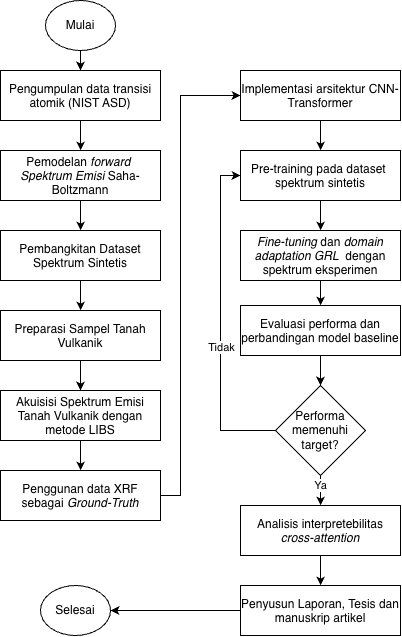
\includegraphics[width=0.55\textwidth]{diagram-alir-M.png}
    \caption{Diagram alir penelitian.}
    \label{fig:diagram-alir}
\end{figure}

\subsection{Prosedur Penelitian, Pengumpulan Data, dan Pengolahan Data}

Prosedur pelaksanaan penelitian ini terdiri dari 4 (empat) tahapan utama yang mendukung rancangan pada diagram alir di atas. Penelitian mengikuti alur kerja yang mengintegrasikan pendekatan fisika eksperimental optik dan teknik \textit{deep learning}, di mana keterbatasan jumlah data eksperimental (24 sampel) diatasi dengan memanfaatkan pengetahuan fisika plasma melalui data sintetis \citep{wang2024, favre2025b} sebelum mentransfer representasi yang telah dipelajari ke domain eksperimental.

% ----------------------------------------------------------------
\subsubsection{Tahap 1: Pembangkitan Data Sintetis}

Keterbatasan utama dalam pengembangan model \textit{deep learning} untuk analisis LIBS adalah minimnya ketersediaan data eksperimental berlabel yang memadai untuk pelatihan. Untuk mengatasi hal ini, penelitian ini memanfaatkan \textit{forward model} berbasis fisika plasma untuk membangkitkan dataset sintetis berskala besar. Pendekatan ini telah terbukti efektif dalam meningkatkan kemampuan generalisasi model melalui \textit{pre-training} pada data sintetis sebelum \textit{fine-tuning} pada data eksperimental \citep{wang2024, favre2025b}. 

Sebelum algoritma numerik dieksekusi, parameter input yang mencakup rentang konsentrasi (\textit{ground-truth} sintetis) dan karakteristik instrumen fisis didefinisikan secara konstan terlebih dahulu. Rentang referensi kelompok elemen penyusun matriks disajikan secara komprehensif pada Tabel~\ref{tab:komposisi-tanah}. Sementara batas variabel simulasi hukum fisikanya dipaparkan secara eksplisit di awal melalui Tabel~\ref{tab:parameter-simulasi}.

\begin{table}[H]
\centering
\caption{Rentang referensi komposisi elemen untuk tanah vulkanik yang digunakan dalam pembangkitan dataset spektral sintetis. Elemen dikelompokkan menjadi elemen mayor dan elemen jejak berdasarkan profil geokimia khas tanah vulkanik dan observasi eksperimental XRF.}
\label{tab:komposisi-tanah}
\small
\begin{tabular}{lllp{6cm}}
\toprule
\textbf{Grup} & \textbf{Elemen} & \textbf{Rentang Komposisi (\%)} & \textbf{Peran / Catatan} \\
\midrule
\multicolumn{4}{l}{\textbf{Elemen Mayor (\textit{Major Elements} --- Komponen matriks utama)}} \\
Mayor & Si & 40 -- 60 & Komponen silikat dominan \\
Mayor & Al & 10 -- 18 & Mineral aluminosilikat / feldspar \\
Mayor & Fe & 5 -- 15 & Oksida besi dan mineral feromagnesia \\
Mayor & Ca & 3 -- 10 & Plagioklas dan mineral karbonat \\
Mayor & Mg & 2 -- 8 & Mineral olivin dan piroksen \\
Mayor & Na & 1 -- 5 & Komponen feldspar alkali \\
Mayor & K & 1 -- 5 & Feldspar kalium \\
Mayor & Ti & 0.5 -- 2 & Mineral oksida (ilmenit / rutil) \\
\midrule
\multicolumn{4}{l}{\textbf{Elemen Jejak (\textit{Trace Elements} --- Elemen minor dan penyerta)}} \\
Jejak & Mn & 0.05 -- 0.5 & Berasosiasi dengan mineral Fe \\
Jejak & P & 0.05 -- 0.5 & Mineral apatit \\
Jejak & Ba & 0.01 -- 0.3 & Elemen jejak asosiasi alkali \\
Jejak & Sr & 0.01 -- 0.2 & Mensubstitusi Ca dalam feldspar \\
Jejak & Zn & 0.005 -- 0.1 & Elemen jejak sulfida / oksida \\
Jejak & Cu & 0.001 -- 0.05 & Logam jejak sulfida \\
Jejak & Ni & 0.001 -- 0.05 & Asosiasi mineral mafik \\
Jejak & Cr & 0.001 -- 0.05 & Indikator mineral ultramafik \\
Jejak & V & 0.001 -- 0.05 & Logam transisi pada mineral mafik \\
Jejak & Rb & 0.001 -- 0.05 & Elemen alkali dalam feldspar \\
Jejak & Pb & 0.001 -- 0.02 & Logam jejak berat \\
Jejak & Co & 0.001 -- 0.02 & Berasosiasi dengan mineral Fe \\
Jejak & Mo & 0.0005 -- 0.01 & Logam jejak minor \\
Jejak & Y & 0.0005 -- 0.01 & Berasosiasi dengan \textit{rare earth element} (REE) \\
Jejak & Zr & 0.001 -- 0.02 & Mineral penyerta zirkon \\
\bottomrule
\end{tabular}
\end{table}

\begin{table}[H]
\centering
\caption{Parameter fisis dan instrumental dalam algoritma pembangkitan data spektrum LIBS sintetis.}
\label{tab:parameter-simulasi}
\small
\begin{tabular}{llp{5.5cm}}
\toprule
\textbf{Kategori / Parameter} & \textbf{Nilai / Rentang} & \textbf{Keterangan} \\
\midrule
Rentang Suhu Elektron ($T_e$) & $6.000 - 15.000$ K & Memodelkan fluktuasi pendinginan plasma \citep{cristoforetti2010} \\
Rentang Densitas Elektron ($n_e$) & $10^{16} - 10^{17}$ cm$^{-3}$ & Menjamin terpenuhinya kriteria \textit{McWhirter} untuk LTE \\
Rentang Spektral ($\lambda$) & $200 - 900$ nm & Penyesuaian batas rentang deteksi \textit{Echelle spectrometer} \\
Resolusi Instrumental (FWHM) & $0{,}02$ nm & Mereplika batasan resolusi optik nyata dari sistem eksperimen \\
Profil Bentuk Garis Emisi & Kurva Voigt & Transisi termal gabungan pelebaran \textit{Doppler} dan \textit{Stark} \\
Fungsi Pelebaran Spektrograf & Distribusi Gaussian & Mendistribusikan piksel menyesuaikan difraksi \textit{grating} alat \\
Total Spektrum Sintetis & $10.000$ set & Varians komprehensif matriks untuk proses \textit{Deep Learning} \\
\bottomrule
\end{tabular}
\end{table}

Setelah pondasi input di atas dipastikan secara ketat, tahapan operasional eksekusi logika pembangkitan data otomatis dikonstruksi secara programatik meliputi langkah berikut:

\begin{enumerate}[label=\arabic*., leftmargin=2cm]
    \item \textbf{Pengumpulan data transisi atomik} diunduh secara algoritmik dari \textit{database} referensi \citep{kramida2024}. Parameter konstan panjang gelombang ($\lambda_{ki}$), Einstein ($A_{ki}$), dan termal nukleus ($E_i$, $g_i$) diseleksi khusus menurut Tabel~\ref{tab:komposisi-tanah}.
    \item \textbf{Penghitungan populasi analit} bersandar penuh pada kesetimbangan termodinamika lokal / LTE. Kalkulasi fraksi status terspesifikasi mengikuti perumusan Distribusi probabilitas keadaan tereksitasi Boltzmann \citep{fujimoto2004}:
    \begin{equation}
        n_{k,z} = n_z \frac{g_{k,z}}{U_z(T_e)} \exp\left(-\frac{E_{k,z}}{k_B T_e}\right)
        \label{eq:boltzmann}
    \end{equation}
    di mana $n_{k,z}$ mewakili agregat spesies di energi mutlak tingkat $k$,  $g_{k,z}$ nilai degenerasi numerik ekuivalen, $U_z$ merujuk agregat partisi termal, dan faktor $k_B$ standar Boltzmann. Kelimpahan proporsi tingkat atom netral dan fraksi ion direkonsiliasi matematis oleh rumusan presisi tinggi \textit{Persamaan Ionisasi Saha}:
    \begin{equation}
        \frac{n_{z+1} n_e}{n_z} = 2 \frac{U_{z+1}(T_e)}{U_z(T_e)} \left(\frac{m_e k_B T_e}{2\pi \hbar^2}\right)^{3/2} \exp\left(-\frac{E_{\infty,z}-\Delta E_{\infty,z}}{k_B T_e}\right)
        \label{eq:saha}
    \end{equation}
    dengan deviasi $\Delta E_{\infty,z}$ mengurangi limit energi normalisasi akibat interferensi ionik yang rapat di volume plasma \textit{screening}. Elemen vital persamaan (*Elektron Temperature* dan *Density*)  disubstitusi otomatis secara acak uniform mematuhi toleransi *sampling* Tabel~\ref{tab:parameter-simulasi}.

    \item \textbf{Pemodelan fungsi spektrum monoatomik ($S_\mathrm{mono}^{(z)}$)}, diformulasikan spesifik tiap analit. Profil kurva \textit{Voigt} dipilih untuk menyeleraskan sebaran tebal intensitas (\textit{Doppler termal} melipat dengan efek turbulensi \textit{Stark elektron}) meniru optika asli difraksi fisik plasma \citep{griem1974}.
    \item \textbf{Campuran komposisi poliatomik multi-konsentrasi}, memproyeksikan fraksi superposisi di seluruh sumbu *wavelength*:
    \begin{equation}
        S_\mathrm{poly}(\lambda) = \sum_{z} c_z \cdot S_\mathrm{mono}^{(z)}(\lambda)
    \end{equation}
    dengan koefisien variabel padat $c_z$ diacak independen sebatas porsi di ambang toleransi Tabel~\ref{tab:komposisi-tanah}. Konstruksi independen dua profil dataset ini yang menjembatani skema pembobotan spesifik arsitektur pengenalan saraf Encoder--Decoder.
    \item \textbf{Validasi final resolusi (\textit{Spline \& Resampling})}, dieksekusi via kernel Gaussian setara (FWHM 0.02 nm) dengan *instrument response function*. Total output kompresi array memformulasikan **10.000 perpaduan spektrum sintetis**, disemai acak dalam partisi stabil 80\% fase *offline training* dan 20\% sebagai data uji hipotesis \textit{Deep Learning}.
\end{enumerate}

% ----------------------------------------------------------------
\subsubsection{Tahap 2: Akuisisi Data Eksperimental}

\paragraph{Sampel Penelitian.}
Penelitian ini memanfaatkan \textbf{24 sampel tanah vulkanik} yang telah dikumpulkan dan dipreparasi dalam rangka program riset kolaboratif grup Laboratorium Optika dan Aplikasi Laser, FMIPA USK. Sampel berasal dari lereng \textbf{Gunung Seulawah Agam, Kabupaten Aceh Besar, Provinsi Aceh}, yang diambil pada \textbf{4 arah mata angin} (Utara, Barat, Selatan, Timur) dan \textbf{3 kedalaman} (0--20 cm, 20--40 cm, 40--60 cm) di setiap titik, sehingga merepresentasikan variasi spasial komposisi geokimia secara sistematis. Strategi pengambilan sampel ini konsisten dengan pendekatan yang digunakan oleh Khumaeni et al. \citep{khumaeni_analysis_2025} pada studi tanah vulkanik Merapi.

Sampel telah dipreparasi menjadi bentuk pelet pada studi sebelumnya melalui prosedur standar:
\begin{itemize}[leftmargin=2cm]
    \item Pengeringan pada suhu ruang untuk menghilangkan kelembaban berlebih.
    \item Penggerusan hingga halus menggunakan mortar dan pestel.
    \item Penyaringan menggunakan ayakan 40 mesh (420 $\mu$m) untuk menyeragamkan ukuran partikel.
    \item Penimbangan sebanyak kurang lebih 3 gram bubuk per sampel.
    \item Pengepresan menggunakan mesin \textit{hydraulic press} dengan tekanan 7 ton selama 5 menit hingga terbentuk pelet dengan ketebalan sekitar 4 mm.
\end{itemize}

Ketersediaan sampel pelet yang telah terpreparasi memungkinkan penelitian ini untuk langsung berfokus pada tahap akuisisi spektrum LIBS baru dan pengembangan model \textit{deep learning}.


\paragraph{Akuisisi Data Spektrum LIBS Baru.}
Meskipun estimasi komposisi (Tabel~\ref{tab:komposisi-tanah}) dan data baseline awal bersumber dari observasi XRF dan CF-LIBS studi terdahulu, standar kualitas data spektral eksperimental masa lalu belum optimal untuk skenario pelatihan komputasi modern. Oleh karena itu, akuisisi spektrum LIBS \textbf{dilakukan secara baru dan independen} terhadap 24 sampel pelet tersebut. Fokus pembaruan eksperimen terletak pada peningkatan agregasi pengukuran: \textbf{jumlah tembakan laser (\textit{shots})} akan diperbanyak secara masif. Penambahan akumulasi tembakan ini sangat esensial untuk mengatasi fluktuasi ketidakstabilan plasma dan menekan profil \textit{noise} temporal. Hasilnya, \textit{Signal-to-Noise Ratio} (SNR) akan meningkat drastis, sehingga jaringan \textit{deep learning} kelak dapat mendeteksi intensitas emisi lemah secara akurat tanpa tertukar dengan \textit{noise}.

Pengukuran dilaksanakan menggunakan sistem LIBS di Laboratorium Optika dan Aplikasi Laser, FMIPA USK. Prosedur pengambilan datanya adalah sebagai berikut:
\begin{itemize}[leftmargin=2cm]
    \item Berkas laser Nd:YAG ($\lambda$ = 1064 nm, energi pulsa 114 mJ) difokuskan pada permukaan sampel pelet menggunakan lensa bikonveks ($f$ = 155 mm) untuk membangkitkan plasma.
    \item Serat optik dihubungkan ke sistem spektrograf dan diarahkan ke bilik sampel untuk menangkap emisi plasma.
    \item Sampel pelet diposisikan di dalam bilik sampel dan jarak fokus disesuaikan untuk memperoleh intensitas plasma yang ideal.
    \item Emisi plasma tertangkap akan direkam menggunakan \textit{Optical Multichannel Analyzer} (OMA) berbasis spektrometer Echelle (rentang 200--900 nm).
    \item Setiap sampel diablasi dengan \textbf{kuantitas tembakan (\textit{multiple shots}) tinggi} pada \textit{crater} / permukaan titik yang berbeda, lalu semua tangkapan spektral dirata-ratakan secara presisi guna memperoleh stabilitas \textit{continuum} \textit{background} dan ketajaman puncak.
    \item Data spektrum yang terekam ditampilkan dan disimpan menggunakan komputer untuk analisis lebih lanjut.
    \item Garis-garis emisi diidentifikasi menggunakan database NIST Atomic Spectra Database \citep{kramida2024}.
\end{itemize}


\paragraph{Data Ground-Truth Konsentrasi (XRF).}
Data konsentrasi elemen untuk seluruh 24 sampel telah tersedia dari pengukuran \textbf{X-Ray Fluorescence (XRF)} yang dilakukan pada studi sebelumnya dalam program riset grup. Data XRF ini digunakan dalam penelitian ini sebagai \textit{ground-truth} konsentrasi unsur untuk supervisi pada tahap \textit{fine-tuning} model. Penggunaan data XRF yang sudah ada memastikan konsistensi referensi antara studi terdahulu dan penelitian ini, serta menghindari pengulangan pengukuran yang tidak diperlukan. XRF dipilih sebagai referensi karena kemampuannya memberikan analisis kuantitatif multi-elemen yang akurat secara non-destruktif.


% ----------------------------------------------------------------
\subsubsection{Tahap 3: Pemodelan \textit{Deep Learning}}

\paragraph{Arsitektur Model CNN--Transformer Encoder--Decoder.}
Arsitektur model yang diusulkan dalam penelitian ini dirancang berdasarkan prinsip dekomposisi spektral mono--poliatomik eksplisit, di mana spektrum campuran poliatomik dimodelkan sebagai superposisi terbobot dari spektrum monoatomik penyusunnya. Secara teknis, rancangan jaringan ini ditunjukkan secara menyeluruh pada Gambar~\ref{fig:arsitektur-cnn-trans}. Arsitektur encoder--decoder dipilih karena secara natural mampu memodelkan hubungan antara komponen individu (monoatomik via encoder) dan campurannya (poliatomik via decoder) melalui mekanisme \textit{cross-attention} \citep{vaswani2017, liu2026}. 

\begin{figure}[htbp]
    \centering
    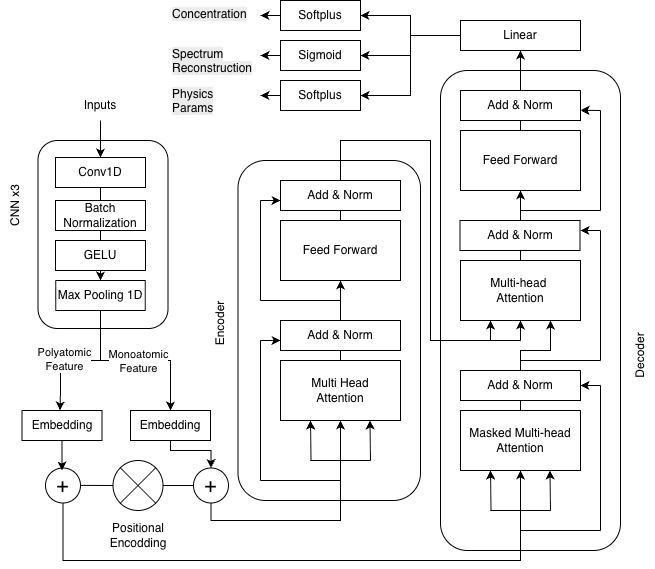
\includegraphics[height=12cm]{Arsitektur-CNN-Trans.png}
    \caption{Representasi visual Arsitektur CNN--Transformer Encoder--Decoder untuk analisis spektral LIBS. Blok ekstrasi fitur 1D CNN dimanfaatkan untuk mereduksi sekuens panjang gelombang sebelum memasuki lapisan atensi Transformer.}
    \label{fig:arsitektur-cnn-trans}
\end{figure}

Komponen utamanya adalah sebagai berikut:

\begin{enumerate}[label=\arabic*., leftmargin=2cm]
    \item \textbf{1D-CNN Feature Extractor} (\textit{shared} encoder--decoder): Dieksekusi secara berulang sebanyak 3 kali blok tumpukan (terdiri dari Conv1D $\rightarrow$ Batch Normalization $\rightarrow$ GELU $\rightarrow$ Max Pooling 1D). Blok ini secara krusial menangkap fitur lokal profil emisi/bentuk garis dan mereduksi resolusi spasial sekuens panjang gelombang.

    \item \textbf{Transformer Encoder} (4 layer, 8 attention heads): menerima fitur CNN dari \textbf{seluruh} spektrum monoatomik (\textit{concatenated}) + \textit{positional} \& \textit{element-type embedding} $\rightarrow$ menghasilkan representasi laten spesifik-elemen via \textit{self-attention}. Encoder mempelajari bagaimana setiap elemen berkontribusi terhadap sinyal spektral secara individual.

    \item \textbf{Transformer Decoder} (4 layer, 8 heads): menerima fitur CNN spektrum campuran poliatomik $\rightarrow$ \textbf{\textit{masked self-attention}} $\rightarrow$ \textbf{\textit{cross-attention}} terhadap output encoder $\rightarrow$ mempelajari aturan komposisi spektral. Mekanisme \textit{cross-attention} memungkinkan decoder untuk meng-query representasi elemen dari encoder dan menentukan kontribusi masing-masing elemen terhadap spektrum campuran yang diamati.

    \item \textbf{Regression Head}: Global Average Pooling $\rightarrow$ Linear projection $\rightarrow$ vektor konsentrasi $\hat{\mathbf{c}} \in \mathbb{R}^Z$.

    \item \textbf{Tiga output head}: (i) konsentrasi elemen (aktivasi Softplus), (ii) rekonstruksi spektrum (Sigmoid), (iii) parameter plasma $T_e$, $n_e$ (Softplus). Desain \textit{multi-task} ini mendorong model untuk tidak hanya memprediksi konsentrasi, tetapi juga mempertahankan konsistensi dengan fisika plasma yang mendasarinya.
\end{enumerate}


\paragraph{Strategi Pelatihan.}
Strategi pelatihan model dirancang dalam tiga fase berurutan untuk memaksimalkan transfer pengetahuan dari domain sintetis ke domain eksperimental. Skema komplit dari alur adaptasi domain ini dapat dilihat pada Gambar~\ref{fig:domain-adapt}.

\begin{figure}[htbp]
    \centering
    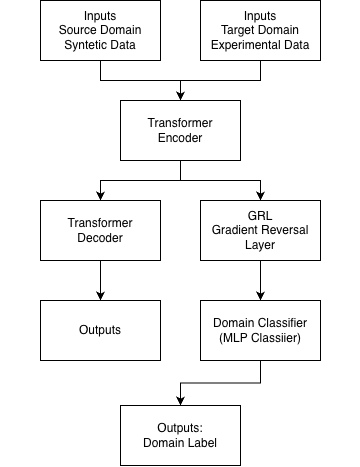
\includegraphics[height=8.5cm]{Domain-Adapt.png}
    \caption{Skema \textit{Domain Adaptation} menggunakan \textit{Gradient Reversal Layer} (GRL). Arsitektur ini memaksa \textit{Transformer Encoder} untuk menghasilkan representasi fitur laten yang tidak bisa dibedakan oleh \textit{Domain Classifier}, sehingga menjembatani \textit{domain gap} antara spektrum sintetis dan eksperimental.}
    \label{fig:domain-adapt}
\end{figure}

\begin{enumerate}[label=\arabic*., leftmargin=2cm]
    \item \textbf{Pre-training} pada data sintetis: 200 epoch, learning rate $10^{-4}$, optimizer Adam \citep{kingma2015} dengan \textit{cosine annealing schedule} \citep{loshchilov2017}. Fungsi loss gabungan digunakan:
    \begin{equation}
        \mathcal{L} = \mathrm{MSE}_\mathrm{konsentrasi} + \alpha \times \mathrm{MSE}_\mathrm{rekonstruksi\;spektral} \quad (\alpha = 0{,}1)
    \end{equation}
    Komponen rekonstruksi spektral berfungsi sebagai regularisasi fisika, memastikan model memetakan fitur spektral yang bermakna secara fisik.

    \item \textbf{Fine-tuning} pada data eksperimental LIBS: 50 epoch, learning rate $10^{-5}$ (lebih rendah untuk mencegah \textit{catastrophic forgetting}), dengan target \textit{ground-truth} konsentrasi dari pengukuran XRF.

    \item \textbf{Domain adaptation}: Gradient Reversal Layer (GRL) \citep{ganin2016} + domain classifier (sintetis vs eksperimental) diintegrasikan selama pelatihan untuk mendorong encoder menghasilkan representasi yang \textit{domain-invariant}. Pendekatan ini mengatasi \textit{domain gap} antara spektrum sintetis (yang mengasumsikan LTE ideal) dan spektrum eksperimental (yang mengandung noise, fluktuasi tembakan-ke-tembakan, dan deviasi dari LTE).
\end{enumerate}


% ----------------------------------------------------------------
\subsubsection{Tahap 4: Analisa Sampel dan Pengolahan Data}

Hasil akuisisi eksperimental dianalisis lebih lanjut melalui serangkaian tahapan komputasional. Pemrosesan data mentah dan analisis luaran model mencakup:
\begin{itemize}[leftmargin=2cm]
    \item \textbf{Pra-pemrosesan spektrum}: normalisasi intensitas terhadap kurva respons sistem (*instrumental response*), koreksi kontinum \textit{baseline} melalui algoritma polynomial fitting, dan segmentasi rentang panjang gelombang fokus untuk membuang \textit{background noise}.
    \item \textbf{Identifikasi garis emisi}: pencocokan otomatis antar puncak profil spektrum yang terukur dengan \textit{database} referensi NIST ASD guna memvalidasi keberadaan matriks elemen target.
    \item \textbf{Inferensi model}: spektrum eksperimental yang telah bersih diumpankan ke model prediksi \textit{deep learning} (CNN--Transformer) yang telah terbiasa dengan spektrum sintetis untuk mengekstrak vektor konsentrasi elemen (\textit{end-to-end mapping}).
    \item \textbf{Analisis komparatif}: penyelarasan keluaran prediksi konsentrasi dari pemodelan AI terhadap perolehan data eksak XRF sebagai landasan validasi metrik (*ground-truth*).
\end{itemize}

\textbf{Protokol Evaluasi Metrik} \\
Evaluasi kapabilitas analitik model dihimpun secara komprehensif menggunakan protokol:
\begin{itemize}[leftmargin=2cm]
    \item \textbf{3 metrik kuantitatif per elemen}: \textit{Root Mean Square Error} (RMSE) untuk melacak rata-rata deviasi kuadratik, \textit{Koefisien Determinasi} ($R^2$) memonitor proporsi korelasi linier prediksi absolut, dan \textit{Mean Absolute Percentage Error} (MAPE) sebagai parameter akurasi relatif spasial.
    \item \textbf{4 model baseline} sebagai komparasi ketangguhan: PLS—\textit{Partial Least Squares} \citep{wold2001} sebagai representasi perbandingan regresi kemometrik klasik, model spasial diskrit (CNN-only), penyesuai sekuens independen (Transformer-only), dan arsitektur canggih \textit{Informer} \citep{zhou2021, walidain2026}.
    \item \textbf{Keterandalan Lintas-Validasi}: \textit{stratified 5-fold cross-validation} diimplementasikan pada dataset eksperimental untuk menihilkan anomali uji (mencegah *overfitting*) serta menyajikan jaminan *robustness* validasi di situasi jumlah sampel yang terbatas.
    \item \textbf{Interpretabilitas Fisik}: penelusuran balik bobot koneksi \textit{cross-attention} dari matriks \textit{decoder} ke \textit{encoder}. Pendekatan ini melegitimasi apakah mesin neural secara mandiri menemukan hubungan spasi-waktu transisi kuantum elemen, menegaskan bahwa simulasi benar-benar mempelajari dekomposisi mono--poliatomik sesuai hukum fisika, bukan sekadar intuisi korelasi statistik "kotak hitam" semata.
\end{itemize}


% ----------------------------------------------------------------
\subsection{Hasil yang Diharapkan}

Dari pelaksanaan penelitian ini, diharapkan diperoleh hasil sebagai berikut:
\begin{enumerate}[label=\arabic*., leftmargin=2cm]
    \item \textbf{Model CNN--Transformer encoder--decoder} yang terlatih dan mampu melakukan kuantifikasi multi-elemen pada spektrum LIBS tanah vulkanik dengan akurasi yang superior dibandingkan model baseline (PLS, CNN-only, Transformer-only, Informer).
    \item \textbf{Validasi konsep dekomposisi spektral mono--poliatomik} melalui analisis bobot \textit{cross-attention}, yang menunjukkan bahwa model secara eksplisit mempelajari kontribusi spektral masing-masing elemen dalam spektrum campuran.
    \item \textbf{Profil konsentrasi 7 elemen mayor} (Si, Al, Fe, Ca, Mg, Na, K) dari 24 sampel tanah vulkanik lereng Gunung Seulawah Agam, Aceh, yang divalidasi terhadap pengukuran XRF.
    \item \textbf{Metode kuantifikasi LIBS baru} yang mengintegrasikan pengetahuan fisika plasma (\textit{physics-informed}) ke dalam arsitektur \textit{deep learning}, membuka peluang analisis geokimia cepat tanpa kalibrasi standar.
    \item \textbf{Manuskrip jurnal ilmiah} yang siap disubmit ke jurnal internasional bereputasi.
\end{enumerate}


% ----------------------------------------------------------------
\subsection{Indikator Capaian yang Ditargetkan}

\begin{itemize}[leftmargin=2cm]
    \item Minimal \textbf{satu publikasi ilmiah} di jurnal internasional bereputasi. Jurnal yang ditargetkan: \textbf{IOP Machine Learning: Science and Technology} (Q1, terindeks Scopus). Sebagai alternatif: \textit{Spectrochimica Acta Part B} atau \textit{Journal of Analytical Atomic Spectrometry}.
    \item \textbf{Penyelesaian tesis} mahasiswa magister dalam rentang waktu yang direncanakan (10 bulan).
    \item \textbf{Peningkatan kapasitas laboratorium} dalam pengembangan dan penerapan metode \textit{deep learning} untuk analisis spektroskopi LIBS, yang dapat digunakan untuk penelitian lanjutan di lingkungan Laboratorium Optika dan Aplikasi Laser, FMIPA USK.
\end{itemize}


% ----------------------------------------------------------------
\subsection{Pembagian Kerja Tim Peneliti dan Keterlibatan Mahasiswa}

\begin{table}[htbp]
\centering
\caption{Pembagian Kerja Tim Peneliti}
\label{tab:tim}
\small
\begin{tabular}{clp{3.5cm}p{6cm}}
\toprule
\textbf{No} & \textbf{Status} & \textbf{Instansi / Bidang} & \textbf{Uraian Tugas} \\
\midrule
1 & Ketua  & FMIPA USK / Optika \& Laser Spektroskopi & Mengkoordinasi pelaksanaan penelitian, mensupervisi pengukuran LIBS dan analisis data, serta mereview manuskrip publikasi \\
\addlinespace
2 & Anggota & FMIPA USK / [Bidang Ilmu] & Supervisi metode komputasi dan pengembangan model \textit{deep learning} \\
\addlinespace
3 & Anggota & FMIPA Fisika USK / Fisika Komputasi \& Spektroskopi & Implementasi arsitektur CNN--Transformer, pembangkitan data sintetis, preparasi sampel, pengambilan data eksperimental LIBS, serta penulisan draf tesis dan manuskrip publikasi \\
\bottomrule
\end{tabular}
\end{table}

\textbf{Keterlibatan Mahasiswa}: Penelitian ini secara esensial adalah subyek dari pengerjaan \textbf{Tesis Magister} yang dilakukan oleh peneliti utama (Mahasiswa). Pembagian kerja di atas memastikan keberlangsungan penelitian ini didukung oleh kepakaran saintifik Promotor (Ketua Peneliti) di bidang instrumen optik laser, dan Co-Promotor (Anggota) di metodologi komputasi, dengan beban eksekusi utama, pengolahan data \textit{deep learning}, serta preparasi lapangan dilimpahkan penuh pada kapasitas intelektual mahasiswa dalam pemenuhan gelar pascasarjana.


% ================================================================

\section{Jadwal Penelitian}
\begin{table}[H]
\centering
\caption{Rencana Jadwal Pelaksanaan Penelitian Tesis}
\small
\begin{tabular}{p{4.5cm}p{1.5cm}p{8cm}}
\toprule
\textbf{Fase} & \textbf{Bulan} & \textbf{Kegiatan Utama} \\
\midrule
1 --- Persiapan Data & 1--3 & Pembangkitan spektrum sintetis (Saha--Boltzmann + NIST ASD), pengumpulan \& preparasi sampel tanah vulkanik, pengukuran XRF \\
2 --- Pengembangan Model & 3--5 & Desain \& implementasi arsitektur CNN--Transformer encoder--decoder \\
3 --- Pelatihan \& Optimasi & 5--8 & Pre-training pada data sintetis, fine-tuning pada data eksperimental, optimasi hyperparameter, domain adaptation \\
4 --- Evaluasi \& Penulisan & 8--10 & Analisis performa, perbandingan baseline, analisis interpretabilitas cross-attention, penulisan tesis \& manuskrip jurnal \\
\bottomrule
\end{tabular}
\end{table}

% ================================================================
\renewcommand{\refname}{Daftar Pustaka}
\bibliographystyle{apalike}
\bibliography{Roadmap/Roadmap,Roadmap/referensi}

\end{document}
